\documentclass[letterpaper, 10pt]{article}

\usepackage{amsmath}
\usepackage{float} 
\usepackage{graphicx}
\usepackage{gensymb}

\usepackage[margin=1in]{geometry}

\title{Radio Background Research Notes}
\author{Nitika Yadlapalli}
\date{}


\begin{document}
\maketitle

\section{Sky Brightness Model for a Disk+Halo and Extragalactic Sources}

\subsection{Contribution from Disk}
Given a pair of galactic coordinates, we need to determine the line of sight through the disk. This, combined with the emissivity of the disk, will allow us to know the flux density contributed by the disk.

\begin{figure}[h]
\begin{center}
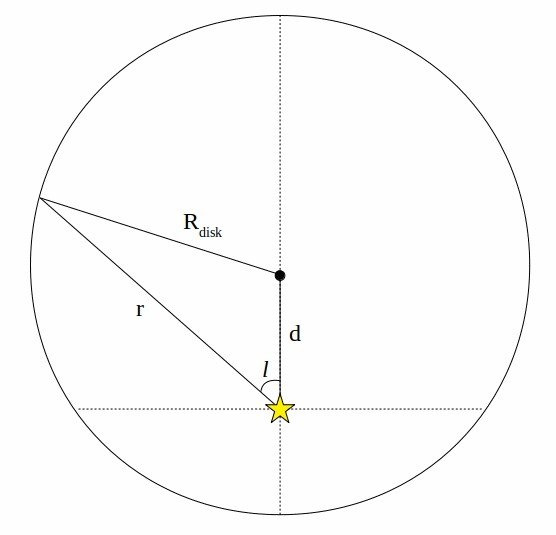
\includegraphics[width=0.39\textwidth]{disk_face.jpg}
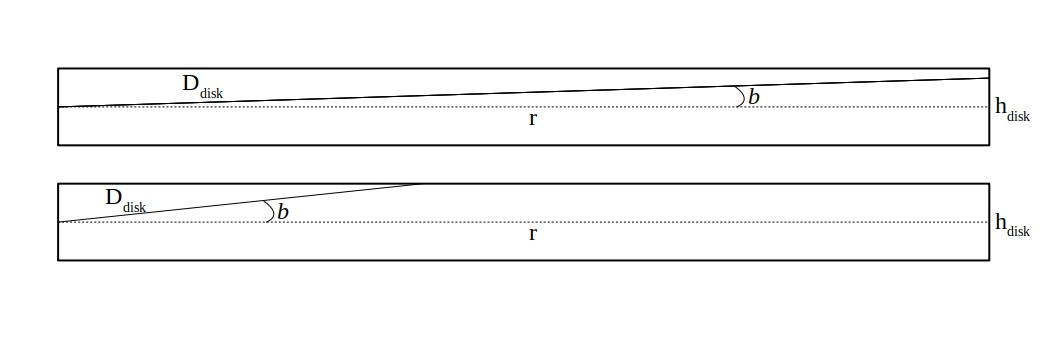
\includegraphics[width=0.59\textwidth]{disk_edge.jpg}
\caption{Two views of disk, face on and edge on, illustrating how line of sight through disk is calculated}
\label{disk}
\end{center}
\end{figure}

\begin{table}[h]
\centering
\begin{tabular}{| c | c |}
\hline
\textbf{Variable} & \textbf{Physical Meaning} \\
\hline
$D_{disk}$ & Total line of sight distance through disk \\
\hline
$R_{disk}$ & Radius of disk \\
\hline
$h_{disk}$ & Height of disk \\
\hline
$d$ & Distance between sun and galactic center \\
\hline
$l$ & Galactic longitude \\
\hline
$b$ & Galactic latitude \\
\hline
$r$ & Intermediate variable \\
\hline
\end{tabular}
\caption{Description of variables shown in Fig~\ref{disk}}
\end{table}

Referring to the left side of Fig~\ref{disk}, the yellow star represents the location of the solar system. The equations presented below will be for $ 0\degree < l < 180\degree $, as the results are symmetric for $ 180\degree < l < 360\degree $. First, making use of law of sines and law of cosines, I find that 

\[ r = \sqrt{R_{disk}^{2} + d^{2} - 2dR_{disk}cos\left[180 - l - sin^{-1}\left(\frac{dsin(l)}{R_{disk}}\right)\right]} \]

Then, given $r$, $D_{disk}$ can be given by one of two equations, depending on the value of $b$. 

\begin{table}[h]\
\centering
\begin{tabular}{c c}
$ D_{disk} = \frac{r}{cos(b)} $ & if $|b| < tan^{-1} \left(\frac{h/2}{r} \right)$ \\

$ D_{disk} = \frac{h}{sin(b)} $ & if $|b| > tan^{-1} \left(\frac{h/2}{r} \right)$ \\

\end{tabular}
\end{table}

Then, given an emissivity for the disk, 
\[F_{\nu, disk} = P_{\nu, disk}D_{disk} \]

In order to check these derived equations, we use example values approximated from the Subrahmanyan and Cowsik paper. A separate analysis will be done later to determine the model parameters that best fit our model to data. The disk model can be verified by plotting $ T_{b}\ vs\ csc(b)$, as shown in Figure~\ref{cscb} below. The plot is linear as expected for a correct model. A map of the brightness contributed just from the disk is shown in Figure~\ref{disk_map}.

\begin{figure}[h]
\begin{center}
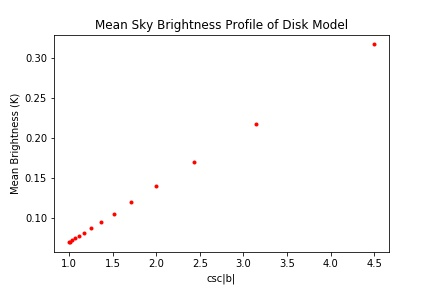
\includegraphics[width=0.5\textwidth]{cscb.jpg}
\caption{Plot of $ T_{b}\ vs\ csc(b)$}
\label{cscb}
\end{center}
\end{figure}

\begin{figure}[h]
\begin{center}
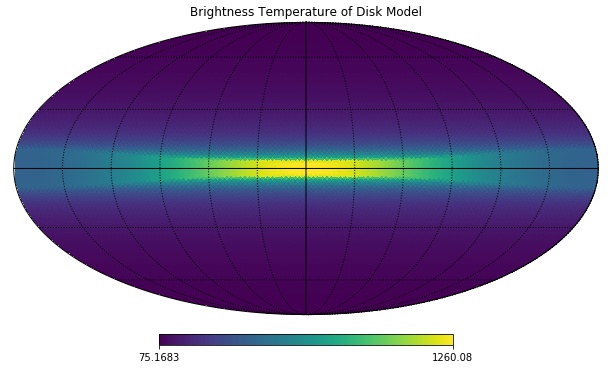
\includegraphics[width=0.6\textwidth]{disk.jpg}
\caption{Map of brightness temperature contributed by the disk}
\label{disk_map}
\end{center}
\end{figure}

\subsection{Contribution from Halo}
Next, we need to calculate the line of sight through the halo. Again, we only concern ourselves with angles in the range $ 0\degree < l < 180\degree $, as it will be symmetric in the range $ 180\degree < l < 360\degree $. To do that, we start by looking at the halo from the face on perspective, relative to the disk. Referring to the left side of Figure~\ref{halo}, we get both $d_{proj}$ and $R_{eff}$, which we need to solve for the entire line of sight through the disk.

\[ d_{proj} = d|cos(l)| \]

For $ l < 90\degree $, 
\[ R_{eff} + d_{proj} = \sqrt{R_{halo}^{2} + d^{2} - 2dR_{halo}cos\left[180 - l - sin^{-1}\left(\frac{dsin(l)}{R_{halo}}\right)\right]} \]

For $ l > 90\degree $, 
\[R_{eff} - d_{proj} = \sqrt{R_{halo}^{2} + d^{2} - 2dR_{halo}cos\left[180 - l - sin^{-1}\left(\frac{dsin(l)}{R_{halo}}\right)\right]} \]


\begin{figure}[h]
\begin{center}
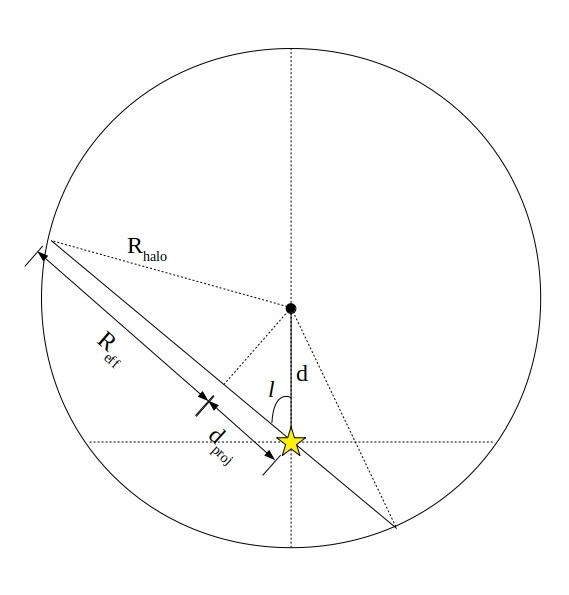
\includegraphics[width=0.495\textwidth]{halo_face.jpg}
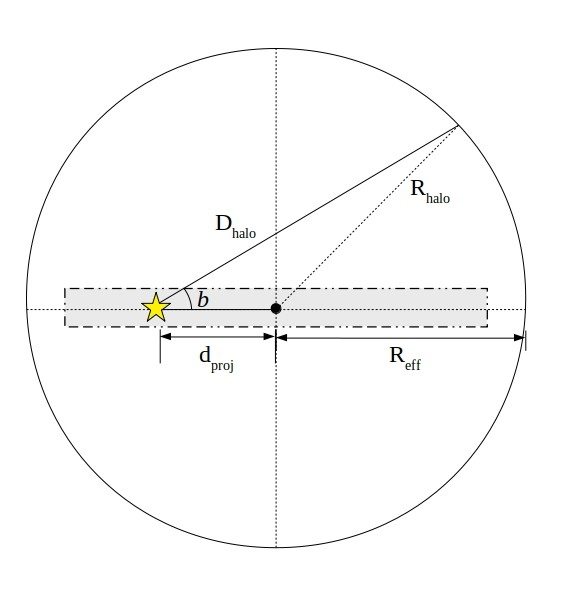
\includegraphics[width=0.485\textwidth]{halo_edge.jpg}
\caption{Two views of halo, face on and edge on (relative to the orientation of the disk), illustrating how line of sight through the halo is calculated. Shown above is an example for $ l < 90\degree$}
\label{halo}
\end{center}
\end{figure}

Next, we look at the halo edge on, relative to the disk, as shown in the right hand side of Figure~\ref{halo}.  For this example, if $ l < 90\degree$, 

\[ D_{halo} = \sqrt{R_{halo}^{2} + d_{proj}^{2} - 2R_{halo}d_{proj}cos\left[180 - b - sin^{-1}\left(\frac{d_{proj}sin(b)}{R_{halo}}\right)\right] }  \]

If $l > 90\degree$, 

\[ D_{halo} = \sqrt{R_{halo}^{2} + d_{proj}^{2} - 2R_{halo}d_{proj}cos\left[b - sin^{-1}\left(\frac{d_{proj}sin(b)}{R_{halo}}\right)\right] }  \]

Then, given an emissivity for the halo, 
\[F_{\nu, halo} = P_{\nu, halo}D_{halo} \]

A map of the brightness contributed just from the halo is shown in Figure~\ref{halo_map}, again using example values taken from the Subrahmanyan and Cowsik paper for the purpose of checking our derived equations.

\begin{figure}[h]
\begin{center}
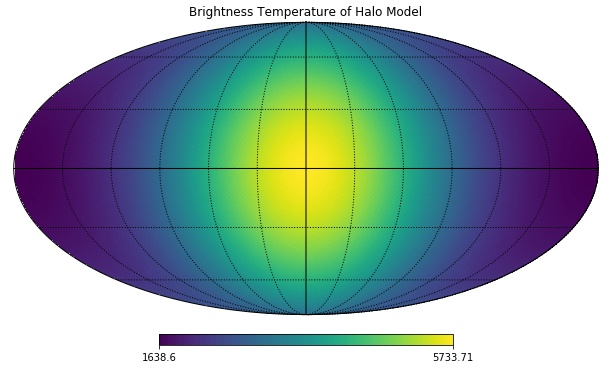
\includegraphics[width=0.6\textwidth]{halo.jpg}
\caption{Map of brightness temperature contributed by the halo}
\label{halo_map}
\end{center}
\end{figure}


\subsection{Extragalactic Source Counts}

Though plots showing source counts spanning over several orders of magnitude of brightness are shown in many papers, the analytic formulas and/or data points are scattered across the literature. In order to get the total sky brightness contributed by extragalactic sources, several models were combined. In the range of $0.05 - 1000\ mJy$ (equivalent to $10^{-5} - 1\ Jy$), can be modelled by the sixth order polynomial described by Hopkins et al (2002). The paper presents the result below, shown both analytically and graphically in Figure~\ref{Hopkins1}. In order to calculate the sky brightness, the curve shown in the right hand plot of Figure 6 must be integrated. 

\[ log\left(\frac{dN/dS}{S^{-2.5}}\right) = -0.008x^{6} + 0.057x^{5} - 0.121x^{4} - 0.049x^{3} + 0.376x^{2} + 0.508x + 0.859 \] \[x = log\left(\frac{S}{mJy}\right) \]

\begin{figure}[h]
\begin{center}
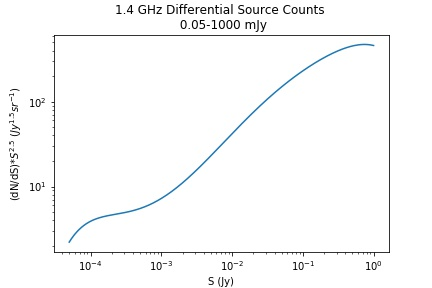
\includegraphics[width=0.49\textwidth]{Hopkins1.jpg}
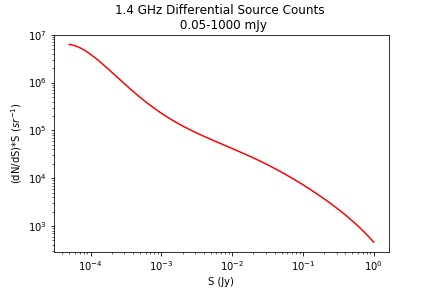
\includegraphics[width=0.49\textwidth]{Hopkins2.jpg}
\caption{Plot showing differential source counts at 1.4 GHz, as modelled in the Hopkins et al 2002 paper, described by $\frac{dN/dS}{S^{-2.5}}$ and a function of $S$ (left), and $S\left(dN/dS\right)$ as a function of $S$ (right), where $S$ is the sky brightness in $Jy$}
\label{Hopkins1}
\end{center}
\end{figure}

In the range of $0.011-44\ mJy$, Smolcic et al (2017), reports specific values for $\frac{dN/dS}{S^{-2.5}}$ at various sky brightnesses. Shown in Figure~\ref{Smolcic} is $S\left(dN/dS\right)$ as a function of $S$. The range of sky brightnesses for which source counts are reported somewhat overlap with the Hopkins paper. As expected, the graphs showing the source counts are consistent with each other.

\begin{figure}[h]
\begin{center}
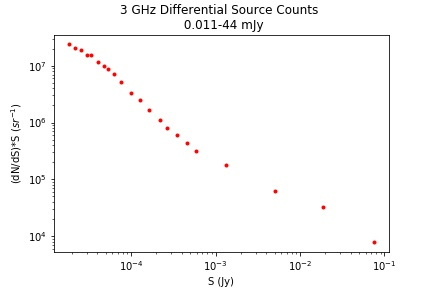
\includegraphics[width=0.49\textwidth]{Smolcic.jpg}
\caption{Plot showing differential source counts at 3 GHz, as modelled in the Smolcic et al (2017) paper, $S\left(dN/dS\right)$ as a function of $S$ }
\label{Smolcic}
\end{center}
\end{figure}

Finally, in the range of $ S < 10\ \mu Jy$, Condon et al 2012 predict that the source counts at 3.02 GHz are described as below. 

\[ \frac{dN}{dS} = 9000S^{-1.7}\ Jy^{-1}\ sr^{-1} \]


\begin{figure}[h]
\begin{center}
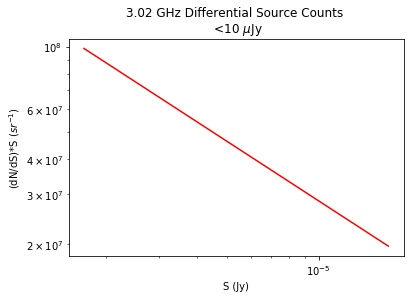
\includegraphics[width=0.49\textwidth]{Condon.jpg}
\caption{Plot showing differential source counts below $10\ \mu Jy$ at 3.02 GHz, as modelled in the Condon et al (2012) paper, $S\left(dN/dS\right)$ as a function of $S$ }
\label{Condon}
\end{center}
\end{figure}

As in this project, we'll be working with models of sky brightness at a particular frequency, we can use the following equation to transform $S$ into the frequency of our choice, where the spectral index is $ \alpha = -0.7$

\[ S_{f} = S_{i} \left(\frac{\nu_{f}}{\nu_{i}}\right)^{\alpha} \]

Total sky brightness is given by 
 \[ S_{tot} = \int \left(S\frac{dN}{dS}\right) dS \]
 
Total brightness temperature is given by the following equation. A plot representing the integrand is shown in Figure~\ref{Tb}.
 \[ T_{b} = \int \left(\frac{dT}{dS}\right) dS \ = \int \left(S\frac{dN}{dS}\right) \frac{c^{2}}{2\nu^{2}k} dS \]
 
\begin{figure}[h]
\begin{center}
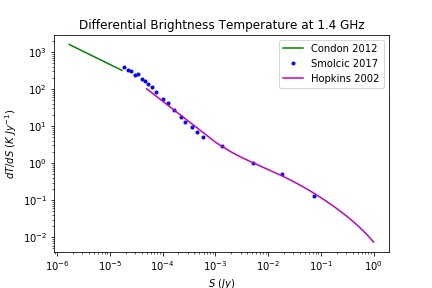
\includegraphics[width=0.59\textwidth]{T_b.jpg}
\caption{Differential brightness temperature plotted as a function of source brightness }
\label{Tb}
\end{center}
\end{figure}


 
\subsection{Masking Pixels in Central Latitudes}

Latitudes between $ -10\degree < b < 10\degree$ include emission from the galactic center that is not well understood. For our analysis, we wish to ignore these regions. Therefore, I have used healpy's pixel querying function to set all of the pixels between these latitudes to zero. The resulting map is shown in Figure~\ref{disk_mod}.

\begin{figure}[h]
\begin{center}
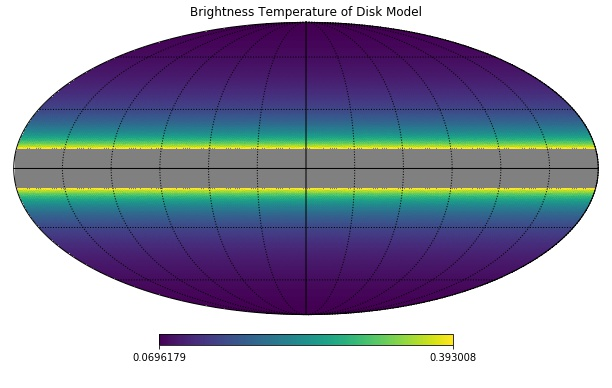
\includegraphics[width=0.6\textwidth]{disk_mod.jpg}
\caption{Map of brightness temperature contributed by the disk, with central latitudes ignored.}
\label{disk_mod}
\end{center}
\end{figure}


\section{Deriving Emissivity from Brightness Temperature}
Given some brightness temperature for both the halo and the disk (such as those given in the Subrahmanyan and Cowsik paper), I want to calculate the the emissivity (power per volume) for the disk and halo. To start, we can use the brightness temperature to calculate specific intensity using the Rayleigh Jeans approximation. 
\[ I_{\nu} = \frac{2\nu^{2}}{c^{2}}kT \]

From the specific intensity, to derive a emissivity, we need to integrate over the solid angle and divide by the length of the line of sight. We can assume that the intensity is constant with respect to the $\phi$ and $\theta$ values in question. All values of brightness temperature in the Subrahmanyan and Cowsik paper are given based on an observer in the galactic center. In the following equation, $\Omega$ is the solid angle and \emph{s} is the length of the line of sight. This will be either $R_{halo}$ or $R_{disk}$.
\[ P_{\nu} = \frac{\Omega I_{\nu}}{s} \]

Given this, the emissivity for the spherical galactic halo is given by 

\[P_{\nu, halo} = (4\pi)\left(\frac{2\nu^{2}}{c^{2}}kT\right)\left(\frac{1}{R_{halo}}\right)\]

while the emissivity for a disk is given by 
\[P_{\nu, disk} = \left[ 2\pi tan^{-1}\left(\frac{h_{disk}}{R_{disk}}\right) \right]\left(\frac{2\nu^{2}}{c^{2}}kT\right)\left(\frac{1}{R_{disk}}\right)\]

Then, the flux density along a line of sight can be given by 

\[F_{\nu} = P_{\nu, halo}D_{halo} + P_{\nu, disk}D_{disk} \]

\end{document}